\section{Objects}
\label{sec:Phase_II_ObjectSel}

Before applying final-state specific category selections, a common set of object selections is required for the various physics objects reconstructed event-by-event for each simulation sample. In order to maximize the number HH events saved, each simulation event is required to have at least one pair of photons, called a diphoton.

Photons used in this analysis are required to have a transverse momentum ($p_T$) above 25 GeV, and at least one photon with a \pt of 35 GeV
within $|\eta| < 2.5$.

The relative isolation of the photon
candidate, defined as sum of the $p_T$ of all particles within a cone ($\Delta R = \sqrt{(\Delta \eta)^2 + (\Delta \phi)^2}$) of size 0.3 around the photon and divided the sum by the photon $p_T$, 
is required to be less than 0.3 and must pass a loose identification criteria corresponding to 90\% signal efficiency.

Electrons are required to have $p_T$ above 10 GeV within $|\eta| < 2.5$ excluding the ECAL transition region and 
must be isolated from photon candidates with an angular separation in the $\eta-\phi$ plane greater than $\Delta R = $ 0.4. 
The transverse momenta of muons are required to be above 10 GeV and within $|\eta| < 2.5$ 
, and they are required to be isolated from photon and electron candidates with an angular separation greater than $\Delta R = $ 0.4. 
Hadronically decaying taus are required to have $p_T >$ 20 GeV within $|\eta| < 2.5$, and are required to be separated from photon, electron and muon candidates  
with an angular separation greater than $\Delta R = $0.2. The relative isolation of the electrons (muons) is required to be less than 0.3 (0.1).

Jets are reconstructed using the anti-$k_{T}$ clustering method with a distance parameter of 0.4. 
They are required to have $p_T >$ 30 GeV, be within $|\eta| < 5$ and to be well separated from the photon and lepton candidates with an angular separation greater than $\Delta R = $ 0.4. The likelihood that a jet comes from b-quark hadronization, termed a b-tagging score, is computed using a deep neural network (DNN) based secondary vertex algorithm, \textsc{Deepjet}~\cite{CMS-DP-2018-058, Bols:2020bkb}. 

\section{Event Selections and Categorization}
\label{sec:Phase_II_Selections}  
All events are required to have exactly two photons with an invariant mass in the range $100 < \mgg < 180$\GeV. The analysis is performed in mutually exclusive final states targeting decays of the vector bosons referred to as 1L (Semi-leptonic) and 2L (Fully-leptonic) final states for \wwgg, and 1 $\tau$ or 2 $\tau$ final states for \ttgg. 

Here, lepton (L) refers to either an electron ($e^{\pm}$) or muon ($\mu^{\pm}$). 

\subsection{Semi-leptonic final state}
\label{sec:oneL} 

Events fall into the Semi-leptonic (1L) analysis category if they contain at least one pre-selected diphoton pair, and contain exactly one electron or muon passing the selection criteria described in Section \ref{sec:Phase_II_ObjectSel}. This final state is expected to be the most sensitive of the three $WW\gamma\gamma$ channels due to the combination of a relatively large $W\rightarrow qq$ branching ratio, and the presence of a highly energy lepton from the $W\rightarrow \ell\nu$ decay. 

In order to maximize the sensitivity of this final state, two multiclass DNNs are trained to separate the di-Higgs signal from the resonant single Higgs boson background and continuum background where the di-Higgs processes are labelled as \textit{HH}, single Higgs backgrounds as \textit{H} and all other background samples as continuum background.

% (HH $\rightarrow$ 2$\gamma 2ql\nu$, HH $\rightarrow$ $2\gamma 2\tau$, HH $\rightarrow 2 \gamma 2l2\nu$) 

During training, each class has a weight applied which scales the event loss such that the effective importance's of each of the three classes are equalized. This ensures that the network focuses on categorising all classes with an equal importance. 

Two multiclass DNNs are trained, one which trains on one half of simulation events, and a second which trains on the other half of simulation events. This separation on simulation datasets allows one to apply the training performed with “even” events on the “odd” data set, and vice versa, to avoid any training bias.

The simulation sample variables used as inputs for the DNN trainings include the kinematic variables such as $p_T$, $\eta$, $\phi$ and energy values of photons, jets, electrons and muons. For photons, $p_T$ and energy values are scaled by the diphoton mass in order to avoid the creation of an artificial resonance among continuum background processes. Additionally, the jet multiplicity, missing transverse energy and the invariant mass of the leading and subleading jets are utilized in the trainings. 

The multiclass DNN outputs three DNN scores, one for each class, but only the HH output DNN score is used in the analysis. The HH DNN score distribution is shown in Figure \ref{fig:oneL_perf}. 

\begin{figure}[!htb]
    \centering
    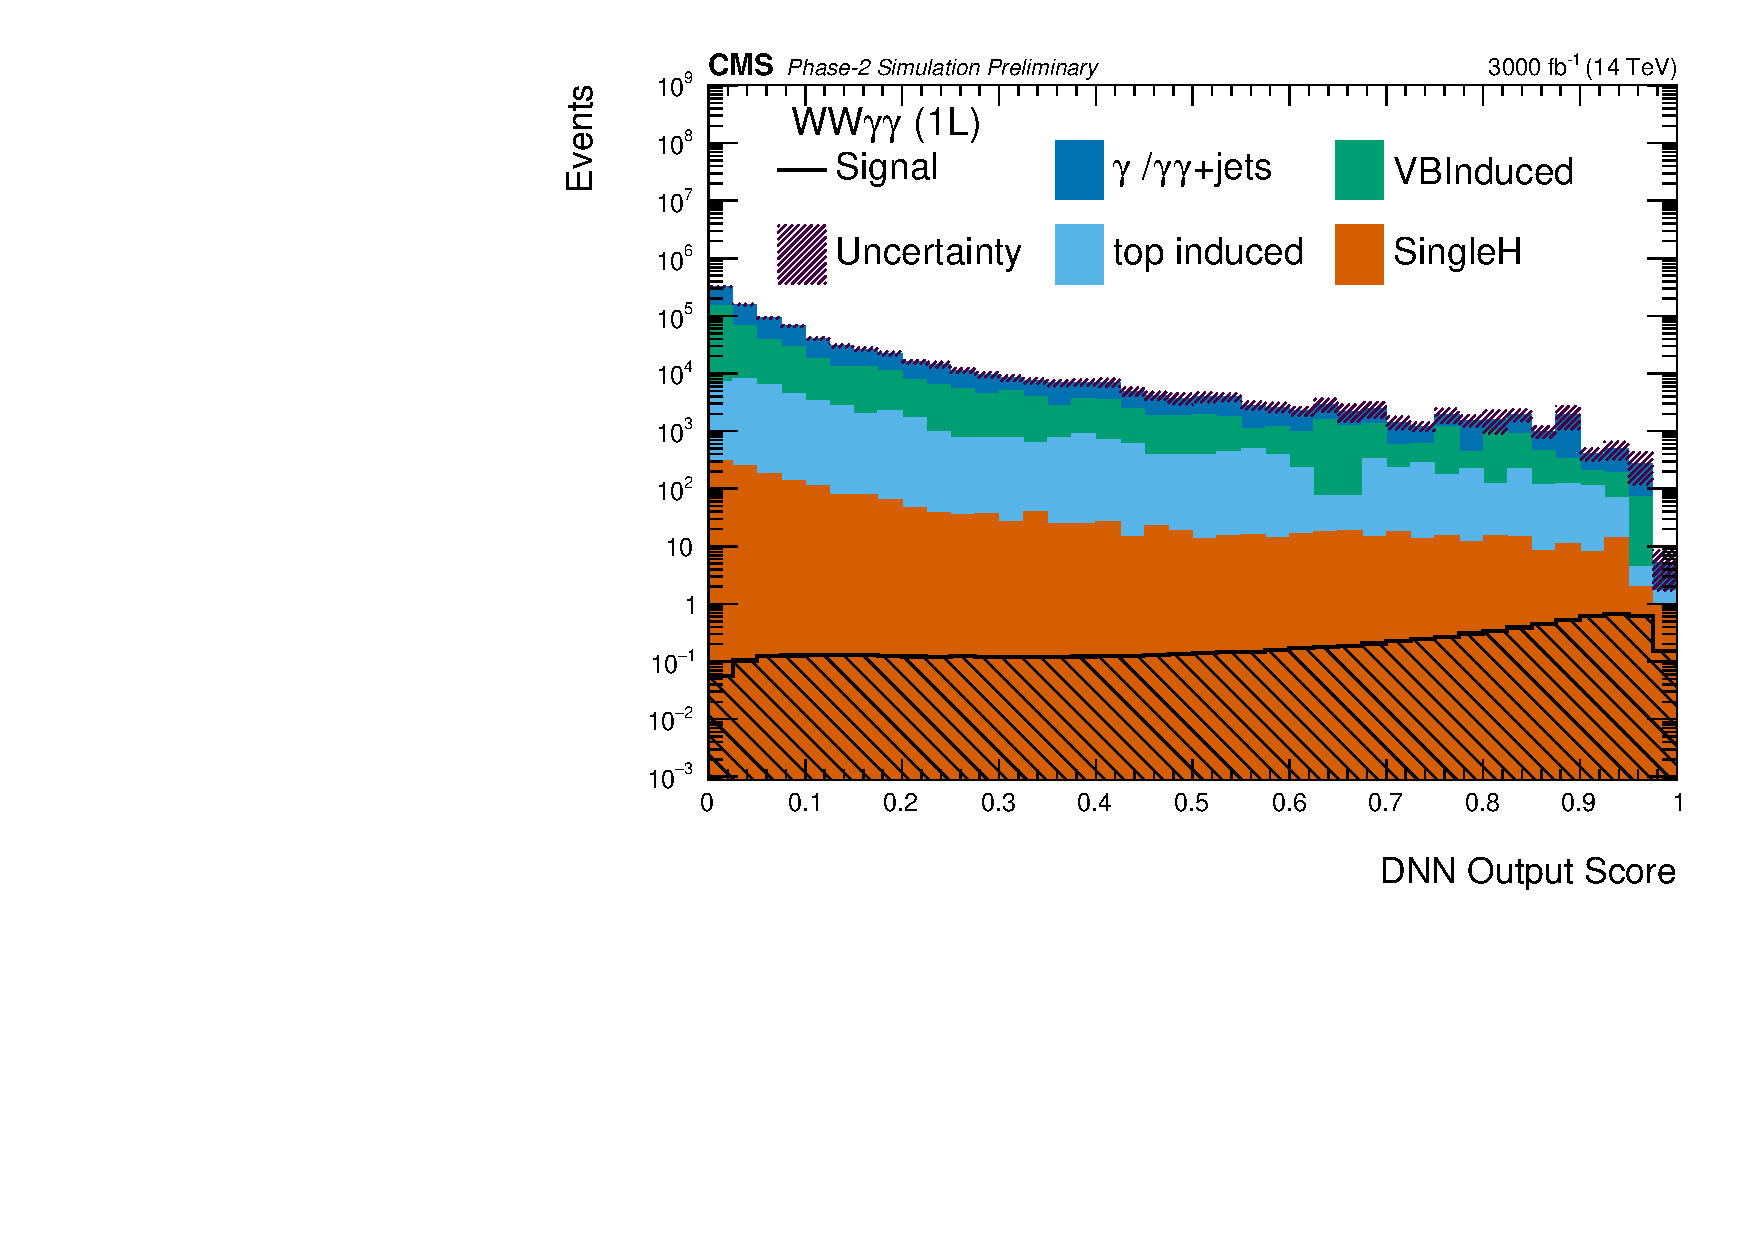
\includegraphics[width=0.75\textwidth]{Sections/Phase_II_HH/images/DNN/DNN_Score_WW_logy.pdf}
    \caption{Semi-leptonic DNN output score distribution.}
    \label{fig:oneL_perf}
\end{figure}

In order to further optimize the analysis sensitivity, events are partitioned into four categories making use of the \textit{HH} node output score. The category boundaries are chosen such that the expected significance is maximized, and are shown in Table \ref{tab:OneLcats}.

\begin{table}[!htb]
  \centering
  \begin{tabular}{ll}
    \hline 
    Categories & Definition\\
    \hline 
    Category 1  & 0.1 $<$ DNN score $<$ 0.6 \\
    Category 2  & 0.6 $<$ DNN score $<$ 0.8 \\
    Category 3  & 0.8 $<$ DNN score $<$ 0.92 \\
    Category 4  & DNN score $>$ 0.92 \\
    \hline
   \end{tabular}
    \caption{
      Semi-leptonic final state DNN score categories.
    }
    \label{tab:OneLcats}
\end{table}

This categorization leads to an improved combined significance as opposed to using a single category, as multiple regions with reasonable signal sensitivities can be combined. Category four is the category with the highest signal purity and significance.  



\subsection{Fully-leptonic final state}
\label{sec:TwoL} 

For events to fall into the Fully-leptonic category, they must contain at least one diphoton candidate, and at least two oppositely charged leptons ($e^+ e^-$, $\mu^+ \mu^-$, $e^{\pm} \mu^{\mp}$)
passing the electron and muon object selections described in Section \ref{sec:Phase_II_ObjectSel}. 

In order to save events with two leptonically decaying W bosons, events fall into the fully-leptonic category if they satisfy the selections listed in Table \ref{tab:FLSelections_Phase_II}, where $\Delta{R(l,l)}$ is the $\Delta{R}$ between two leptons, $m_{ll}$ is the mass of dilepton system and $m_{e\gamma}$ is the invariant mass of the leading electron and the leading photon in the events that have at least one electron. 

\begin{table}[!h]
    \begin{center}
        \begin{tabular}{c|c}
        Variable & Selection \\ \hline
        $\Delta{R(l,l)}$ & $> 0.4$ \\
        \pt of leading lepton & $> 20\GeV $\\
        \pt of subleading lepton & $> 10\GeV$ \\
        $E_T^{miss}$ & $> 20\GeV$ \\
        $p_T^{\gamma\gamma} $ & $> 91 \GeV$ \\
        $m_{ll}$ & $<80 \GeV$ or $>100 \GeV $ \\
        number of medium-tagged b-jets & $ = 0 $ \\
        $|m_{e\gamma} - m_{z}|$ & $ > 5\GeV$ \\
        %Third lepton veto (No third lepton with \pt) & $> 10 \GeV$ \\
        \end{tabular}
    \end{center}
    \caption{
      Selection criteria of the Fully-leptonic Channel.
    }
    \label{tab:FLSelections_Phase_II}
\end{table}
\subsection{One Tau lepton final state}
\label{sec:oneT}

Events fall into the one $\tau$ category if they contain at least one diphoton candidate, 
exactly one hadronically decaying tau lepton, and exactly zero electrons and muons. 

In order to maximize the sensitivity of this final state, a similar method to that of the semi-leptonic final state described in Section \ref{sec:oneL} is followed. Namely, two multiclass deep neural networks (DNNs) are trained. In this case, the structure of the DNNs are the same as those from the semi-leptonic analysis, with the electron and muon input features replaced by the $\tau$ candidate's input features. The multiclass DNNs output three scores, but only the one which estimates the likelihood that an event is HH like is used in this analysis. The distribution of this DNN score is shown in Figure \ref{fig:tau_perf}.

\begin{figure}[!htb]
    \centering
    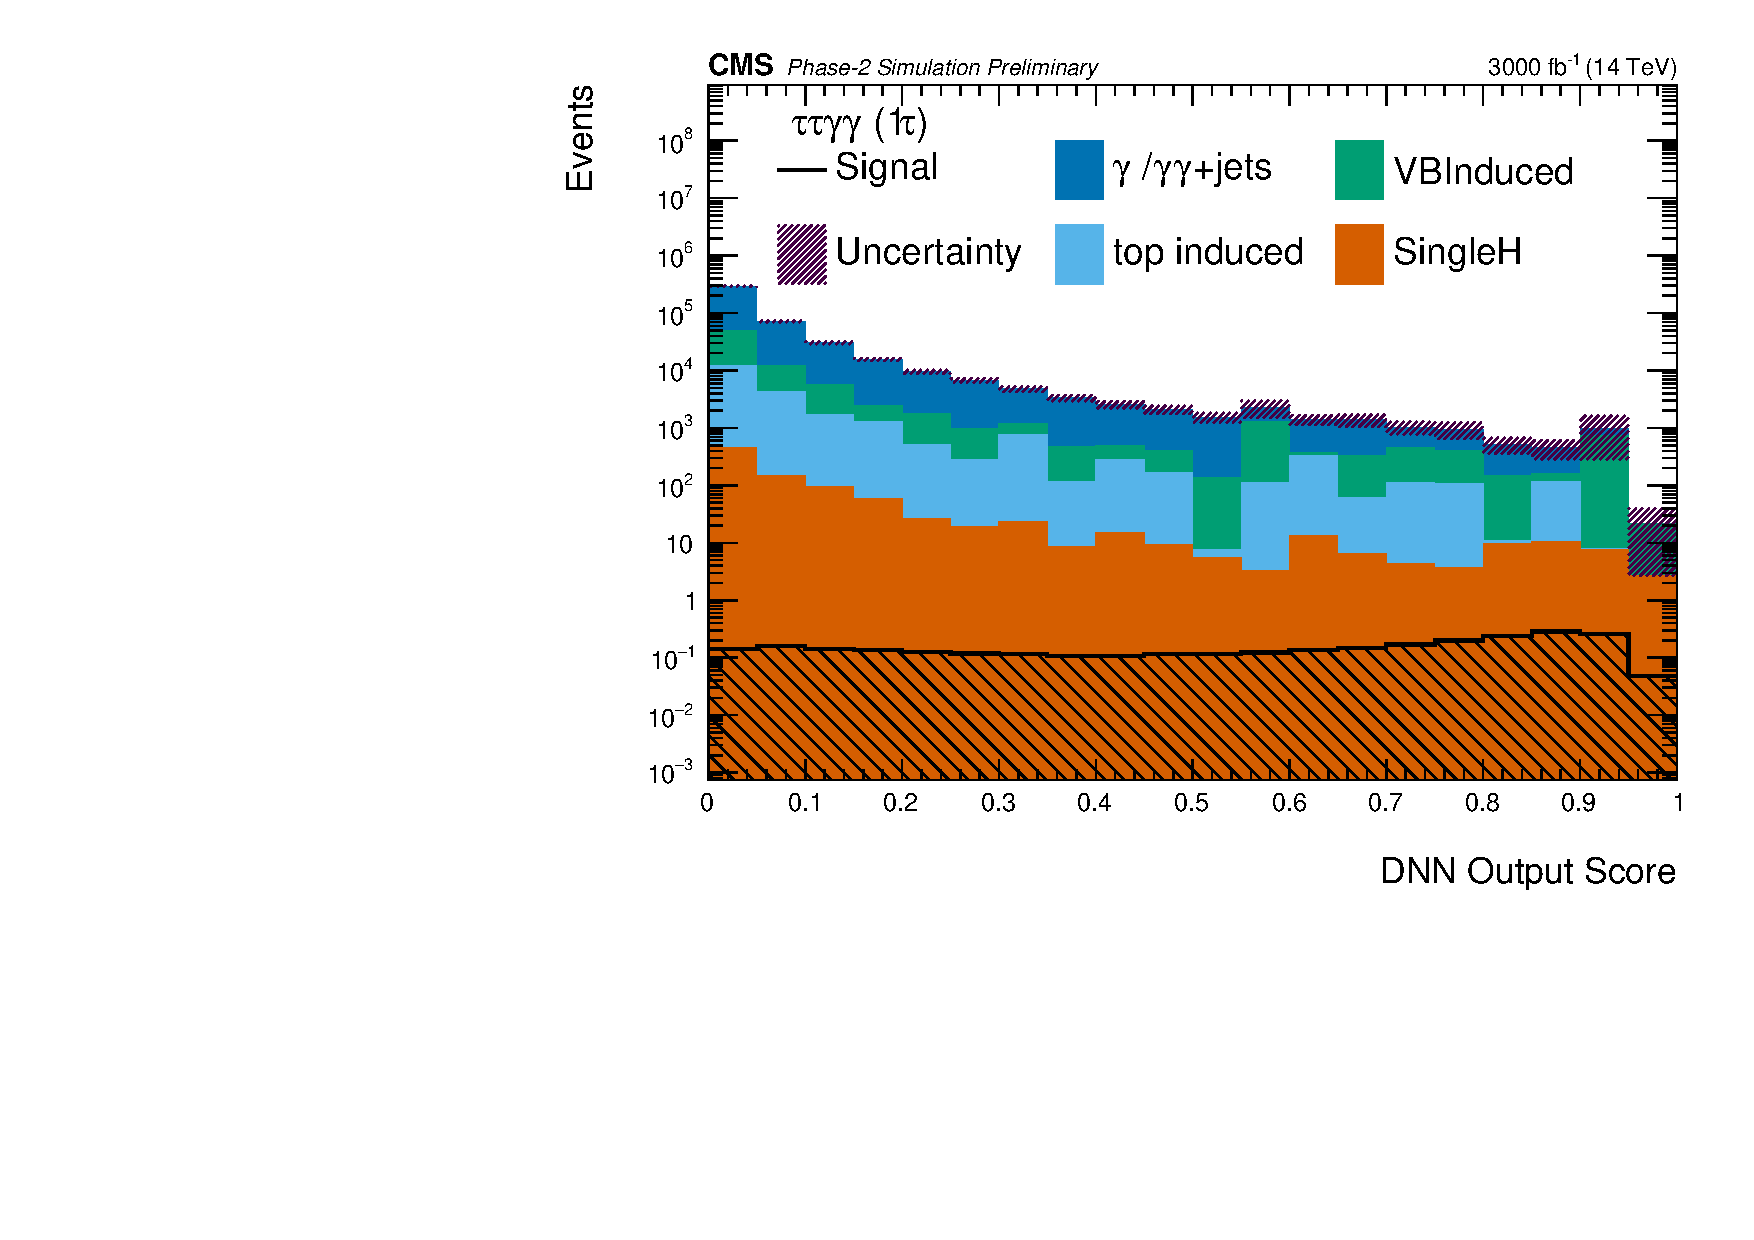
\includegraphics[width=0.75\textwidth]{Sections/Phase_II_HH/images/DNN/DNN_Score_tt_logy.pdf}
    \caption{One tau DNN output score distribution.}
    \label{fig:tau_perf}
\end{figure}

Events are partitioned into two categories based on the DNN score. Category one corresponds to events where the DNN score lies between 0.1 and 0.65, while events with a DNN score higher than 0.65 are placed into category 2. 




\subsection{Two Tau leptons final state}

Events fall into the two $\tau$ final state if they contain at least one diphoton candidate, at least two hadronically decaying taus, and zero electrons and photons. For the taus, it is required that they be oppositely charged because they are expected to come from a neutral Higgs boson. In this final state category, no additional selections are required. 